% Erlang Trace Debugging
% Compile with: xelatex erlang_trace_debugging.tex (run twice for TOC)
\documentclass[a4paper,11pt]{article}

% ============================================================
% Packages
% ============================================================
\usepackage{fontspec}
\usepackage{xeCJK}
\setCJKmainfont[BoldFont=STHeiti, ItalicFont=STKaiti]{STSong}
\setCJKsansfont{STHeiti}
\setCJKmonofont{STFangsong}

\usepackage[margin=2.5cm]{geometry}
\usepackage{graphicx}
\usepackage{xcolor}
\usepackage{hyperref}
\usepackage{listings}
\usepackage{booktabs}
\usepackage{longtable}
\usepackage{enumitem}
\usepackage{tikz}
\usepackage{tcolorbox}
\usepackage{fancyhdr}
\usepackage{titlesec}
\usepackage{amsmath}
\usepackage{amssymb}
\usepackage{float}
\usepackage{tabularx}
\usepackage{multirow}
\usepackage{array}

\usetikzlibrary{arrows.meta, positioning, shapes.geometric, fit, calc, backgrounds}

\tcbuselibrary{listings, skins, breakable}

% ============================================================
% Color Definitions
% ============================================================
\definecolor{erlred}{HTML}{A4070A}
\definecolor{erlblue}{HTML}{2B5EA7}
\definecolor{erlgreen}{HTML}{2E7D32}
\definecolor{erlyellow}{HTML}{F9A825}
\definecolor{erlpurple}{HTML}{6A1B9A}
\definecolor{codebg}{HTML}{F5F5F5}
\definecolor{codeborder}{HTML}{CCCCCC}
\definecolor{tipbg}{HTML}{E8F5E9}
\definecolor{warnbg}{HTML}{FFF3E0}
\definecolor{notebg}{HTML}{E3F2FD}
\definecolor{darkgray}{HTML}{333333}

% ============================================================
% Hyperref Setup
% ============================================================
\hypersetup{
    colorlinks=true,
    linkcolor=erlblue,
    urlcolor=erlpurple,
    citecolor=erlgreen,
    pdftitle={Erlang Trace Debugging},
    pdfauthor={Erlang Study Notes},
    bookmarksnumbered=true,
}

% ============================================================
% Code Listing Style
% ============================================================
\lstdefinelanguage{erlang}{
    morekeywords={module, export, import, behaviour, behavior, spec, type,
        record, define, include, ifdef, ifndef, else, endif, undef,
        case, of, end, if, receive, after, when, fun, try, catch, throw,
        begin, spawn, spawn_link, register, self, send, ok, error,
        true, false, undefined, infinity, timeout, noreply, reply, stop,
        hibernate, ignore, normal, process_flag, trap_exit, monitor_node,
        trace, trace_pattern, flush, all, call, return_to, procs, send,
        garbage_collection, timestamp, running, arity, global, local,
        meta, set_on_spawn, set_on_link, existing, new, tracer},
    sensitive=true,
    morecomment=[l]{\%},
    morestring=[b]",
    morestring=[b]',
}

\lstdefinestyle{erlangstyle}{
    language=erlang,
    basicstyle=\ttfamily\small,
    keywordstyle=\color{erlblue}\bfseries,
    commentstyle=\color{erlgreen}\itshape,
    stringstyle=\color{erlred},
    numberstyle=\tiny\color{gray},
    numbers=left,
    numbersep=8pt,
    backgroundcolor=\color{codebg},
    frame=single,
    rulecolor=\color{codeborder},
    breaklines=true,
    breakatwhitespace=true,
    tabsize=4,
    showstringspaces=false,
    captionpos=b,
    xleftmargin=1.5em,
    framexleftmargin=1em,
    aboveskip=1em,
    belowskip=0.8em,
}

\lstdefinestyle{shellstyle}{
    basicstyle=\ttfamily\small\color{white},
    backgroundcolor=\color{darkgray},
    rulecolor=\color{darkgray},
    frame=single,
    breaklines=true,
    showstringspaces=false,
    xleftmargin=1.5em,
    framexleftmargin=1em,
    aboveskip=1em,
    belowskip=0.8em,
}

\lstset{style=erlangstyle}

% ============================================================
% Custom tcolorbox Environments
% ============================================================
\newtcolorbox{tipbox}[1][]{
    colback=tipbg, colframe=erlgreen!80!black,
    fonttitle=\bfseries, title={#1},
    arc=2mm, boxrule=0.8pt,
    left=6pt, right=6pt, top=4pt, bottom=4pt,
    breakable,
}

\newtcolorbox{warnbox}[1][]{
    colback=warnbg, colframe=erlyellow!80!black,
    fonttitle=\bfseries, title={#1},
    arc=2mm, boxrule=0.8pt,
    left=6pt, right=6pt, top=4pt, bottom=4pt,
    breakable,
}

\newtcolorbox{notebox}[1][]{
    colback=notebg, colframe=erlblue!80!black,
    fonttitle=\bfseries, title={#1},
    arc=2mm, boxrule=0.8pt,
    left=6pt, right=6pt, top=4pt, bottom=4pt,
    breakable,
}

% ============================================================
% Graphics path
% ============================================================
\graphicspath{{images/}}

% ============================================================
% Header / Footer
% ============================================================
\pagestyle{fancy}
\fancyhf{}
\fancyhead[L]{\small\textit{Erlang Trace Debugging}}
\fancyhead[R]{\small\textit{RabbitMQ Source Analysis}}
\fancyfoot[C]{\thepage}
\renewcommand{\headrulewidth}{0.4pt}

% ============================================================
% Title Formatting
% ============================================================
\titleformat{\section}
    {\LARGE\bfseries\color{erlblue}}
    {\thesection}{1em}{}[\vspace{-0.5em}\rule{\textwidth}{0.8pt}]

\titleformat{\subsection}
    {\Large\bfseries\color{erlblue!80!black}}
    {\thesubsection}{0.8em}{}

\titleformat{\subsubsection}
    {\large\bfseries\color{erlblue!60!black}}
    {\thesubsubsection}{0.6em}{}

% ============================================================
% Document Begin
% ============================================================
\begin{document}

% ---- Title Page ----
\begin{titlepage}
\centering
\vspace*{3cm}

{\fontsize{42}{48}\selectfont\bfseries\color{erlblue} Erlang Trace}\\[12pt]
{\fontsize{24}{28}\selectfont\color{erlblue!70!black} Debugging}

\vspace{2cm}

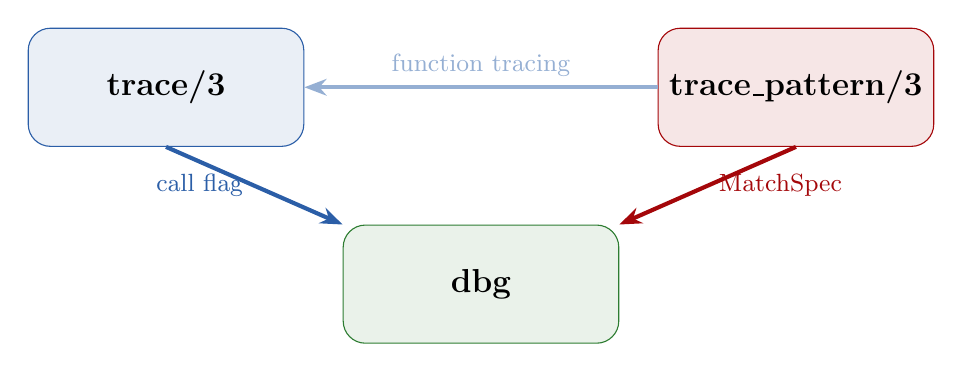
\begin{tikzpicture}
    \node[draw=erlblue, fill=erlblue!10, rounded corners=8pt, minimum width=3.5cm, minimum height=1.5cm, font=\large\bfseries] (trace) at (0,0) {trace/3};
    \node[draw=erlred, fill=erlred!10, rounded corners=8pt, minimum width=3.5cm, minimum height=1.5cm, font=\large\bfseries] (pattern) at (8,0) {trace\_pattern/3};
    \node[draw=erlgreen, fill=erlgreen!10, rounded corners=8pt, minimum width=3.5cm, minimum height=1.5cm, font=\large\bfseries] (dbg) at (4,-2.5) {dbg};

    \draw[-{Stealth[length=8pt]}, line width=1.5pt, erlblue]
        (trace.south) -- node[left, font=\small] {call flag} (dbg.north west);
    \draw[-{Stealth[length=8pt]}, line width=1.5pt, erlred]
        (pattern.south) -- node[right, font=\small] {MatchSpec} (dbg.north east);
    \draw[{Stealth[length=8pt]}-, line width=1.5pt, erlblue!50]
        (trace.east) -- node[above, font=\small] {function tracing} (pattern.west);
\end{tikzpicture}

\vspace{3cm}

{\large\color{darkgray} RabbitMQ Source Analysis --- Erlang Trace Debugging}

\vspace{1cm}

{\normalsize\color{gray} trace $\cdot$ trace\_pattern $\cdot$ dbg $\cdot$ recon}

\vfill
{\small\today}
\end{titlepage}

% ---- Table of Contents ----
\newpage
\tableofcontents
\newpage

% ============================================================
% Section 1: Introduction
% ============================================================
\section{开场介绍}

不同语言的调试方式对比：

\begin{itemize}[leftmargin=1.5em]
    \item \textbf{C/C++}: GDB 单步调试
    \item \textbf{Java}: IDE (Eclipse / IntelliJ IDEA)
    \item \textbf{Erlang}: 进程级别的 trace 调试
\end{itemize}

\subsection{资料介绍}

\subsubsection{书籍介绍}

\begin{itemize}[leftmargin=1.5em]
    \item \href{https://drive.weixin.qq.com/s?k=AJEAIQdfAAoNQ4m0keAIUAewaBACc}{\textit{erlang in anger.pdf}}
    \item \href{https://www.erlang-in-anger.com/}{Stuff Goes Bad: Erlang in Anger}
\end{itemize}

\begin{figure}[H]
\centering

\includegraphics[width=0.3\textwidth]{image1}\hfill

\includegraphics[width=0.3\textwidth]{image2}\hfill

\includegraphics[width=0.3\textwidth]{image3}
\caption{Erlang in Anger 书籍封面}
\end{figure}

\begin{figure}[H]
\centering

\includegraphics[width=0.85\textwidth]{image4}
\caption{Erlang 调试相关论文与资料}
\end{figure}

\begin{itemize}[leftmargin=1.5em]
    \item \href{https://www.academia.edu/113957930/Declarative_debugging_of_concurrent_Erlang_programs}{Declarative debugging of concurrent Erlang programs}
    \item \href{https://www.researchgate.net/publication/220178306_Trace_Analysis_of_Erlang_Programs}{Trace Analysis of Erlang Programs}
    \item \href{https://esl-conf-static.s3.eu-central-1.amazonaws.com/media/files/000/000/725/original/Peter_Gomori_-_Profiling_and_Tracing_for_all_with_Xprof.pdf?1503506041}{Profiling and Tracing for all with Xprof}
    \item \href{https://www.amazon.com/Erlang-Programming-Concurrent-Approach-Development/dp/0596518188}{Erlang Programming: A Concurrent Approach to Software Development}
\end{itemize}

\subsubsection{dbg 资料}

\begin{itemize}[leftmargin=1.5em]
    \item \href{https://drive.weixin.qq.com/s?k=AJEAIQdfAAoXAN8Ii8AIUAewaBACc}{dbg.pdf}
    \item \href{https://www.erlang-factory.com/upload/presentations/316/dbg[1].pdf}{dbg - Erlang Factory}
\end{itemize}

% ============================================================
% Section 2: Overview of Erlang Debugging Tools
% ============================================================
\section{Erlang 的调试工具整体介绍}

\begin{figure}[H]
\centering

\includegraphics[width=0.85\textwidth]{image5}
\caption{Erlang 调试工具全景}
\end{figure}

\begin{figure}[H]
\centering

\includegraphics[width=0.85\textwidth]{image6}
\caption{调试工具与 trace flags 对应关系}
\end{figure}

\subsection{trace 介绍}

\begin{figure}[H]
\centering

\includegraphics[width=0.85\textwidth]{image7}
\caption{trace BIF 介绍}
\end{figure}

\subsection{trace 的功能介绍}

trace 能够跟踪三大类事件：

\begin{enumerate}[leftmargin=1.5em]
    \item \textbf{与进程相关的活动和消息传递}
    \item \textbf{垃圾回收和内存使用}
    \item \textbf{全局和本地函数调用}
\end{enumerate}

\begin{figure}[H]
\centering

\includegraphics[width=0.5\textwidth]{image8}\hfill

\includegraphics[width=0.4\textwidth]{image9}
\caption{trace 功能分类}
\end{figure}

事件类型、工具和 trace flag 的对应关系：

\begin{table}[H]
\centering
\renewcommand{\arraystretch}{1.4}
\begin{tabularx}{\textwidth}{>{\bfseries}l X >{\bfseries}l}
\toprule
\textbf{事件类型} & \textbf{工具} & \textbf{trace Flag} \\
\midrule
与进程相关的活动和消息传递 & trace, dbg, redbug & all $|$ send $|$ 'receive' $|$ procs, running 等 \\
\midrule
垃圾回收和内存使用 & trace, dbg, redbug & garbage\_collection $|$ timestamp 等 \\
\midrule
全局和本地函数调用 & trace + trace\_pattern, dbg, redbug, recon\_trace & call $|$ arity $|$, return\_to 等 \\
\bottomrule
\end{tabularx}
\caption{事件类型与 trace flag 对照表}
\end{table}

% ============================================================
% Section 3: API Introduction
% ============================================================
\section{API 介绍}

\subsection{erlang:trace/3 概述}

\begin{itemize}[leftmargin=1.5em]
    \item 调试器和进程管理器等工具使用这个 BIF 来收集和显示跟踪事件
    \item 跟踪事件以以下格式的消息发送：
\end{itemize}

\begin{lstlisting}
{trace, Pid, Tag, Data1 [,Data2]}
\end{lstlisting}

其中 \lstinline|[,Data2]| 表示依赖于跟踪消息类型的可选字段。生成的跟踪事件包括：

\begin{itemize}[leftmargin=1.5em]
    \item 全局和本地函数调用
    \item 垃圾回收和内存使用
    \item 与进程相关的活动和消息传递
\end{itemize}

\begin{notebox}[核心要点]
也就是除了跟踪函数，还能跟踪进程和内存。
\end{notebox}

\subsection{关键注意事项}

\begin{warnbox}[tracer process 不能被跟踪]
调用 \lstinline|erlang:trace(self(), Bool, TraceFlags)| 会产生一个错误的参数错误，因为\textbf{跟踪器进程 tracer process 不能被跟踪}。
\end{warnbox}

\begin{itemize}[leftmargin=1.5em]
    \item 如果你想让其他进程（而不是调用 \lstinline|trace/3| BIF 的进程）接收跟踪事件，你可以将 \lstinline|{tracer, Pid}| 元组作为 \lstinline|TraceFlags| 列表中的一个元素传递。在这个元组中，\lstinline|Pid| 必须是一个进程或端口标识符。
    \item \lstinline|erlang:trace/3| 调用的\textbf{返回值是一个整数}，表示被跟踪的进程数量。
\end{itemize}

\begin{notebox}[基础函数]
\lstinline|erlang:trace/3| 是一个会被其它所有的跟踪工具使用到的函数。

\href{https://erlang.org/doc/man/erlang.html#trace-3}{erlang:trace/3} is the tracing function that all other tracing tools are built on.

If no tracer is specified, the calling process receives all the trace messages.
\end{notebox}

% ============================================================
% Section 4: Process and Port Tracing
% ============================================================
\section{进程和端口追踪}

进程和端口追踪 --- 与进程相关的活动和消息传递。

\begin{figure}[H]
\centering

\includegraphics[width=0.85\textwidth]{image10}
\caption{进程追踪 trace flags}
\end{figure}

\subsection{send \&\& 'receive'}

\subsubsection{send}

\begin{lstlisting}
{trace, PidPort, send, Msg, To}
\end{lstlisting}
When \lstinline|PidPort| sends message \lstinline|Msg| to process \lstinline|To|.

\begin{lstlisting}
{trace, PidPort, send_to_non_existing_process, Msg, To}
\end{lstlisting}
When \lstinline|PidPort| sends message \lstinline|Msg| to the non-existing process \lstinline|To|.

\subsubsection{'receive'}

\begin{lstlisting}
{trace, PidPort, 'receive', Msg}
\end{lstlisting}
When \lstinline|PidPort| receives message \lstinline|Msg|. If \lstinline|Msg| is set to \lstinline|time-out|, a receive statement can have timed out, or the process received a message with the payload \lstinline|timeout|.

\subsection{一些解释注意事项}

\subsubsection{返回信息的格式}

\begin{itemize}[leftmargin=1.5em]
    \item \textbf{当前进程}：如果不指定 tracer，则调用进程充当 tracer，接收所有的 trace 信息
    \item \textbf{trace 不能跟踪 tracer 本身}
\end{itemize}

\begin{figure}[H]
\centering

\includegraphics[width=0.85\textwidth]{image11}
\caption{trace 返回信息格式 (1)}
\end{figure}

\begin{figure}[H]
\centering

\includegraphics[width=0.7\textwidth]{image12}
\caption{trace 返回信息格式 (2)}
\end{figure}

\subsubsection{trace 之后的消息}

trace 之后的消息是进程信息，从一个进程发送到另一个进程的 mailbox 中。既然是一个独立的进程来跟踪事件，所以必然是发送消息的方式。

\begin{figure}[H]
\centering

\includegraphics[width=0.85\textwidth]{image13}
\caption{trace 消息传递机制 (1)}
\end{figure}

\begin{figure}[H]
\centering

\includegraphics[width=0.8\textwidth]{image14}
\caption{trace 消息传递机制 (2)}
\end{figure}

\begin{figure}[H]
\centering

\includegraphics[width=0.7\textwidth]{image15}
\caption{trace 消息传递机制 (3)}
\end{figure}

\subsubsection{如果是终端，需要 flush()}

跟踪事件是以消息的方式出现，如果是终端收到消息，则需要 flush。

\begin{warnbox}[特别注意：终端要 flush 才能看到]
\textbf{This flush() flushes the process mailbox and not the io buffer.}
\end{warnbox}

\subsection{trace 的 PidSpec --- 进程信息}

\begin{description}[leftmargin=1.5em]
    \item[all] All currently existing processes and all processes that will be created in the future.
\end{description}

\subsection{进程相关的 trace 的 FlagList}

\subsubsection{all --- 跟踪所有标志位}

\textbf{all} --- Set all trace flags except \lstinline|{tracer, Tracer}| and \lstinline|cpu_timestamp| that are in their nature different than the others.

\subsubsection{mailbox messages --- 跟踪 send, 'receive'}

\subsubsection{进程跟踪 --- procs}

\lstinline|set_on_spawn|、\lstinline|set_on_link| 等必须结合 \lstinline|procs| 来使用，否则不生效。

\begin{figure}[H]
\centering

\includegraphics[width=0.85\textwidth]{image16}
\caption{procs flag 与 set\_on\_spawn / set\_on\_link}
\end{figure}

\subsubsection{running and exiting}

\subsubsection{选项是叠加的}

这里对 \lstinline|[set_on_spawn, procs]| 和 \lstinline|[running, procs]| 进行了叠加。

\subsection{垃圾回收和内存使用 --- garbage\_collection}

\begin{tipbox}[提示]
占用内存太小，可能触发不到垃圾回收。
\end{tipbox}

\begin{lstlisting}
erlang:trace(Pid, true, [garbage_collection, timestamp]).
erlang:trace(Pid, true, [garbage_collection, timestamp, procs]).
\end{lstlisting}

% ============================================================
% Section 5: trace && trace_pattern Function Tracing
% ============================================================
\section{trace \&\& trace\_pattern 函数追踪}

\subsection{整体介绍}

\begin{figure}[H]
\centering

\includegraphics[width=0.85\textwidth]{image6}
\caption{trace 与 trace\_pattern 配合}
\end{figure}

事件类型与工具、FlagList 的对应关系：

\begin{table}[H]
\centering
\renewcommand{\arraystretch}{1.4}
\begin{tabularx}{\textwidth}{>{\bfseries}l >{\bfseries}l X}
\toprule
\textbf{事件类型} & \textbf{工具} & \textbf{FlagList} \\
\midrule
与进程相关的活动 & trace & all $|$ send $|$ 'receive' $|$ procs 等 \\
\midrule
垃圾回收和内存使用 & trace & garbage\_collection 等 \\
\midrule
全局和本地函数调用 & trace\_pattern & call $|$ arity $|$ return\_to 等 \\
\bottomrule
\end{tabularx}
\caption{事件类型与 FlagList 对照表}
\end{table}

更详细的对照（含 MatchSpec）：

\begin{table}[H]
\centering
\renewcommand{\arraystretch}{1.4}
\begin{tabularx}{\textwidth}{>{\bfseries}l >{\bfseries}l >{\bfseries}l X}
\toprule
\textbf{事件类型} & \textbf{工具} & \textbf{FlagList} & \textbf{MatchSpec} \\
\midrule
全局和本地函数调用 & trace & call, arity, return\_to & --- \\
\midrule
全局和本地函数调用 & trace\_pattern & global, local, meta & return\_trace (返回值) \\
\bottomrule
\end{tabularx}
\caption{trace 与 trace\_pattern 详细对照表}
\end{table}

\begin{figure}[H]
\centering

\includegraphics[width=0.85\textwidth]{image17}
\caption{trace\_pattern 说明 (1)}
\end{figure}

\begin{figure}[H]
\centering

\includegraphics[width=0.85\textwidth]{image18}
\caption{trace\_pattern 说明 (2)}
\end{figure}

\subsection{call (trace FlagList)}

\subsection{global $|$ local (trace\_pattern FlagList)}

\begin{itemize}[leftmargin=1.5em]
    \item 默认值为 \lstinline|global|
    \item \lstinline|local| --- 追踪本地函数调用
\end{itemize}

\begin{warnbox}[注意事项]
\begin{itemize}
    \item 只使用 \lstinline|trace| 或者 \lstinline|trace_pattern| 是不生效的
    \item 必须先启动程序或者先 \lstinline|l(Module)|，再调用 \lstinline|trace_pattern|，否则也不生效
    \item \lstinline|return_to| 可以结合 \lstinline|local| 使用
\end{itemize}
\end{warnbox}

\subsection{return\_to (trace FlagList)}

\begin{notebox}[return\_to 要点]
\begin{itemize}
    \item \textbf{只对 local 选项生效} --- Only works for functions traced with option \textbf{local} to \lstinline|erlang:trace_pattern/3|.
    \item \textbf{return\_to 无法获取函数返回值} --- 如果要取得返回值，在 match specification 中使用 \lstinline|{return_trace}|
\end{itemize}
\end{notebox}

\subsection{return\_trace (trace\_pattern MatchSpec)}

ActionFunction ::= \lstinline|set_seq_token| $|$ \lstinline|get_seq_token| $|$ \lstinline|message| $|$ \lstinline|return_trace| $|$ \lstinline|exception_trace| $|$ \lstinline|process_dump| $|$ \lstinline|enable_trace| $|$ \lstinline|disable_trace| $|$ \lstinline|trace| $|$ \lstinline|display| $|$ \lstinline|caller| $|$ \lstinline|caller_line| $|$ \lstinline|current_stacktrace| $|$ \lstinline|set_tcw| $|$ \lstinline|silent|

获取函数的返回值的追踪信息，在 MatchSpec 中指定 \lstinline|{return_trace}|。

\subsection{return\_to 与 return\_trace 的区别}

\begin{warnbox}[注意事项]
\begin{itemize}
    \item \lstinline|return_to| 和 \lstinline|return_from| 是相互独立的
    \item \lstinline|return_to| 是由 \lstinline|erlang:trace/3| 的 flag 指定的
    \item \lstinline|return_from| 是由 \lstinline|erlang:trace_pattern/3| 的 MatchSpec 指定的
\end{itemize}
\end{warnbox}

\subsection{arity (trace FlagList)}

\begin{itemize}[leftmargin=1.5em]
    \item 使用 \lstinline|arity| 返回的是参数个数
    \item 不使用 \lstinline|arity|，返回的是参数
    \item 如果对参数不感兴趣，或者减小消息大小，使用 \lstinline|arity|
\end{itemize}

\subsection{trace\_pattern/3 的 FlagList 其他选项}

\begin{figure}[H]
\centering

\includegraphics[width=0.85\textwidth]{image19}
\caption{trace\_pattern FlagList 选项 (1)}
\end{figure}

\begin{figure}[H]
\centering

\includegraphics[width=0.85\textwidth]{image20}
\caption{trace\_pattern FlagList 选项 (2)}
\end{figure}

\begin{figure}[H]
\centering

\includegraphics[width=0.85\textwidth]{image21}
\caption{trace\_pattern FlagList 选项 (3)}
\end{figure}

\subsection{匹配规则 Match Specifications}

结合 dbg 一起讲解。

\textbf{MatchSpecList} --- A list of match specifications. An empty list is equivalent to \lstinline|true|. See the ERTS User's Guide for a description of match specifications.

\begin{itemize}[leftmargin=1.5em]
    \item \href{https://erlang.org/documentation/doc-7.0/erts-7.0/doc/html/match_spec.html}{Erlang -- Match specifications in Erlang}
\end{itemize}

\begin{figure}[H]
\centering

\includegraphics[width=0.85\textwidth]{image22}
\caption{Match Specifications 语法}
\end{figure}

\begin{itemize}[leftmargin=1.5em]
    \item \href{https://www.erlang.org/doc/man/dbg.html#fun2ms-1}{Erlang -- dbg:fun2ms/1}
\end{itemize}

MS functions are written as \lstinline|function()|; E.g. \lstinline|message()| and \lstinline|return_trace()|, etc.

\begin{figure}[H]
\centering

\includegraphics[width=0.85\textwidth]{image23}
\caption{dbg:fun2ms 用法}
\end{figure}

\subsection{trace\_pattern 备份 --- 函数追踪}

\subsubsection{函数追踪 call}

Tracing Calls with the \lstinline|trace_pattern| BIF:

You use the \lstinline|erlang:trace_pattern/3| BIF to enable tracing of local and global function calls.

\begin{figure}[H]
\centering

\includegraphics[width=0.85\textwidth]{image24}
\caption{trace\_pattern 函数追踪}
\end{figure}

\subsection{trace\_pattern 的一些总结}

\begin{notebox}[trace\_pattern 要点]
\begin{itemize}
    \item \textbf{trace\_pattern 专门跟踪 exported functions，结合 call 来使用}

    This BIF is used to enable or disable call tracing for exported functions. It must be combined with \href{https://erlang.org/doc/man/erlang.html#trace-3}{erlang:trace/3} to set the \lstinline|call| trace flag for one or more processes. (manual)

    \item \textbf{trace/3 和 trace\_pattern/3 的配合}

    Using \lstinline|trace/3|, you define which processes you want to monitor. Using \lstinline|trace_pattern/3|, you define the subset of functions you are tracing. An event will be generated only if a traced process executes a traced function.
\end{itemize}
\end{notebox}

\subsubsection{return\_to 返回值}

这个选项是 \lstinline|trace/3| 的，不是 \lstinline|trace_pattern/3| 的，要特别注意。

You can use the \lstinline|return_to| flag only in conjunction with the \lstinline|call| flag.

\begin{warnbox}[特别注意]
\textbf{只追踪 local 函数，不追踪 global}

This trace message is sent if both the \lstinline|call| and the \lstinline|return_to| flags are set, and the function is set to be traced on \textbf{local} function calls.

\textbf{其实这个 return\_to 是一个 local 函数，并非 loop}
\end{warnbox}

\subsubsection{可以使用 Arity}

如果对参数不感兴趣，或者减小消息大小，使用 \lstinline|arity|。

\subsubsection{需要先 load module}

The modules we are passing to \lstinline|erlang:trace_pattern/3| have to be loaded before the BIF is called. 类似 \lstinline|l(ping)|.

\subsubsection{global 和 local 选项的区别}

\begin{itemize}[leftmargin=1.5em]
    \item local 调用
    \item global 调用
\end{itemize}

Running the same tests gives you a trace message, namely the one generated as a result of the \lstinline|spawn/3| BIF.

But if you are tracing all global calls in all processes, why did \lstinline|ping:send/1| not generate a trace event? It is, after all, a global call.

\textbf{The reason is that the process receiving the trace messages cannot be traced.}

\subsubsection{如何重定向到其他进程？}

If you want to generate trace events for the process calling the trace BIF, you have to redirect these messages to another process. You do so by passing the \lstinline|{tracer, Pid}| option to the \lstinline|trace/3| BIF, specifying the pid of the process you want to send the messages to.

参考：\href{http://stratus3d.com/blog/2021/08/24/guide-to-tracing-in-erlang/}{Guide to Tracing in Erlang - Stratus3D}

\subsubsection{return\_trace / return\_value}

To get trace messages containing return values from functions, use the \lstinline|{return_trace}| match\_spec action instead.

% ============================================================
% Section 6: Trace Summary
% ============================================================
\section{trace 的一些总结}

\begin{enumerate}[leftmargin=1.5em]
    \item \textbf{erlang:trace/3 位于 runtime system，是 low-level 的}

    The built-in function \lstinline|erlang:trace/3| enables and disables the low-level trace mechanisms in the Erlang runtime system.

    \item \textbf{trace event 是通过发送 message 的方式来的}

    Trace events are sent as messages of the following format:
    \begin{lstlisting}
{trace, Pid, Tag, Data1 [,Data2]}
    \end{lstlisting}

    \item \textbf{trace 事件包含的信息} --- trace events that are generated include the following:
    \begin{itemize}
        \item Global and local function calls
        \item Garbage collection and memory usage
        \item Process-related activities and message passing
    \end{itemize}

    \item \textbf{只有一个进程能够接收 trace event}，注意是消息 message，这个进程叫做 \textbf{tracer process}

    At any one time, only one process may receive trace events from another process. This is known as the tracer process. The tracer process that receives the trace events is the one that made the call to:
    \begin{lstlisting}
erlang:trace(PidSpec, Bool, TraceFlags).
    \end{lstlisting}

    \item \textbf{用特定的进程跟踪消息}

    If you want a process other than the one calling the trace/3 BIF to receive the trace events, you pass the \lstinline|{tracer, Pid}| tuple as an element in the TraceFlags list.

    \item \textbf{return\_to} --- 仅用于 \lstinline|trace/3|，只对 local 函数生效

    \item \textbf{trace 可以重复调用吗，是覆盖还是追加？}

    \item \textbf{send 和 receive 的返回格式}

    \item \textbf{生成一个进程永远不会失败，失败的是进程执行函数的时候}

    Remember, spawning a process never fails. Instead, what fails is the newly spawned process, as the function it is supposed to execute is undefined.

    \item \textbf{trace 返回被 trace 的进程的数量}

    Note how commands return the integer 1, namely the number of processes that are being traced.

    \item \textbf{trace 的时机} --- 既可以是进程生成之前，也可以是之后

    生成之前：using the \lstinline|all| or \lstinline|new| flag. \\
    生成之后：using the \lstinline|all| or \lstinline|existing| flag or the flag's process identifier.

    \item \textbf{函数跟踪}

    如果要跟踪函数，那么必须结合 \lstinline|erlang:trace_pattern/3| 来使用。
    \begin{lstlisting}
call  Trace certain function calls. Specify which
      function calls to trace by calling
      erlang:trace_pattern/3.
Message tags: call, return_from.
    \end{lstlisting}

    \item \textbf{跟 call flag 一起使用的标志位} --- You can use the \lstinline|return_to| flag only in conjunction with the \lstinline|call| flag.
\end{enumerate}

参考链接：

\begin{itemize}[leftmargin=1.5em]
    \item \href{https://www.erlang.org/doc/man/erlang.html#trace-3}{Erlang -- erlang:trace/3}
    \item \href{https://doc.weixin.qq.com/doc/w3_AIUAewaBACc4ilDrxT9SjibA28sn2?scode=AJEAIQdfAAojdOKAc0AIUAewaBACc}{erlang debug 调试技术 sys dbg recon}
    \item \href{https://doc.weixin.qq.com/doc/w3_AIUAewaBACcTot3IcVWQGOwFVxt4b?scode=AJEAIQdfAAoVnq1gYcAIUAewaBACc}{trace \& trace\_pattern}
    \item \href{https://doc.weixin.qq.com/doc/w3_AIUAewaBACcCD0oSSjeRWq9zYIkDY?scode=AJEAIQdfAAoMSomy0mAIUAewaBACc}{dbg}
    \item \href{https://doc.weixin.qq.com/doc/w3_AIUAewaBACcB8Sc5GZ7R2ON9VMb12?scode=AJEAIQdfAAoG04EhcxAIUAewaBACc}{recon}
\end{itemize}

\begin{notebox}[注意]
trace 的 manual 在 erlang 分节。recon\_trace 它只能追踪函数调用，而不能追踪消息。
\end{notebox}

% ============================================================
% Section 7: dbg
% ============================================================
\section{dbg}

\begin{figure}[H]
\centering

\includegraphics[width=0.85\textwidth]{image25}
\caption{dbg 概述}
\end{figure}

\begin{itemize}[leftmargin=1.5em]
    \item 内置函数 trace
    \item dbg 建立在内置函数上
\end{itemize}

用 dbg 调试 dbg 本身，看是不是走的 trace。

\end{document}
